\documentclass[12pt]{article}

\title{Research paper}
\author{Wessel Stoop, s0808709}

\usepackage{covington}
\usepackage{graphicx}
\usepackage{natbib}

\renewcommand{\familydefault}{\sfdefault}

\begin{document}
\maketitle

\section{Introduction}

When one of Starfleet's vessels meets an alien ship in areas where no man has gone before, they can (almost) always communicate with these aliens (almost) instantly; they speak to them in English, and these aliens answer in English. This is possible because, according to the Star Trek lore, the protagonists make use of a so-called Universal Translator. This Universal Translator can (1) recognize speech in every language, (2) translate what it has 'heard' to any other language, (3) make its results audible with speech synthesis and (4) learn itself new languages when needed. Unfortunately, like many technologies in Star Trek, this is far from reality: there is lots of active research at the first three tasks in particular (and even some of the fourth, see \citet{biemann11}), but no software currently in existence can do this as perfect as the Universal Translator. \\\indent
In this paper, I will give a detailed overview of the research project Colibri, which basically is an attempt to improve the technology needed for the second task: automatically translating text from one language to another. More specifically, the project investigates the identification and extraction of constructions in natural language, and how these can be used in Machine Translation. These constructions can be of various lengths, and, importantly, can also contain one or more gaps. The constructions are not identified on the basis of explicit 'human' knowledge about language and grammar ('linguistic theory'), but are distilled from large amounts of text ('text corpora') with the help of context-sensitive machine-learning techniques. The Colibri project is carried out by Maarten van Gompel and supervised by Antal van den Bosch.
\\\indent
In section 2, I'll give a short overview of what has been achieved in machine translation, and in section 3 the current project will be described. This order was chosen to show that Colibri builds on previous research directly.

%Rest van de beschrijving.







\section{Theoretical background / framework}

In this section I will try to give a short overview of the various approaches in machine translation, with special attention to the example-based approach, as that is the approach used in this project. This section is mainly based on \citet{vangompel09}

\subsection{The rule-based approach}

The rule-based approach, also known as Classical Machine Translation, is best characterized by the use of human created rules. That is, authors of translation algorithms tried to include their knowledge about the languages and translation. The rule-based approach can be subdivided into four subapproaches, summarized in the Vauquois triangle: \\

\begin{figure}[htb]
\centering
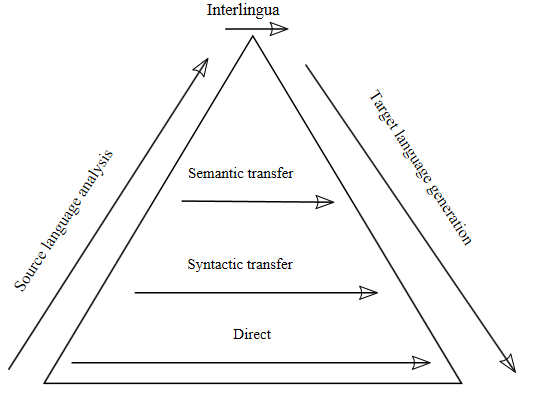
\includegraphics[width=0.8\textwidth]{vauquois.png}
\caption{The Vauquois triangle}
\label{fig:vauquois}
\end{figure}

The horizontal arrows represent the approaches. I'll go through them from bottom to top:

\begin{itemize}
\item \emph{The direct approach} does very little source language analysis, and could thus be viewed as the automatical version of looking up every word in the source language in a dictionary and replacing it with the corresponding word in the target language. This often doesn't yield very good results: if I for example would have translated this paper from my mother tongue Dutch to English word for word, 'would we now not real a good result have'. It should be noted, however, that the direct approach mostly is more complicated than this; for example, in some cases morphological analysis is needed before it can be looked up in a dictionary, and more morphological analysis is needed for the translation word to fit in the sentence. Word reordering rules can also be included.
\item \emph{The syntactic approach} tries to find out the syntactic structure of the source sentence before it starts translating, using a parser. This structure is then translated to the target language, and filled with translated words.
\item \emph{The semantic approach} goes even one step further and also tries to grasp the meaning of a sentence, roughly. For a sentence like /emph{Mummy kisses daddy} this for example entails that mummy is the agent, and daddy the patient of the sentence. After having identified these semantic roles, the algorithm would then look how this meaning is expressed in the target language, find the approriate syntactic structure for that, and fill it with the translated words.
\item \emph{The interlingua approach}. All of the approaches so far have in common that they require a seperate rule set for each language pair; no or very few rules included for translations from English to German can also be used for translations from English to French. The Interlingua approach is an attempt to solve this problem, by pairing up every language with a formal representation of meaning, the Interlingua. This means a translation from English to German would entail a translation from English to the Interlingua (using the ruleset English $\rightarrow$ Interlingua) and then a translation from the Interlingua to German (using the ruleset Interlingua $\rightarrow$ German). When translating from English to French, the same two steps would be taken, and the same ruleset English $\rightarrow$ Interlingua can be re-used. 
\end{itemize}

An advantage of the rule-based approach is that one has a lot of control over the output. In theory, if something has gone wrong, all one has to do is find out which rule or dictionary item caused the problem and improve it. In practice, however, it is almost impossible to have a dictionary and rule system good enough for more complicated sentences, and things like rule interactions and ambiguity make everything even more complicated. The next two approaches therefore replace hand-crafted rules with automatically generated ones.

% Voorbeelden? References?

\subsection{The statistical approach}

Unlike the ruled-based approach, the statistical approach creates its own 'knowledge', using bilingual text corpora. With this knowledge, the algorithm is able to generate various translation hypotheses, from which the best one is chosen with the help of various statistical measures. I will explain these stages in more detail:

\begin{itemize}
\item \emph{Corpus alignment.} Only having a bilingual corpus is not enough: for such a corpus to be useful one also needs to know which parts of the sentence in language A correspond to which part of the sentence B. This is not only complicated by different word orders, but also by concepts that in language A take more or less words than in language B. A well-known word alignment algorithm that tries to solve this problem is the Expectation Maximisation algorithm \citep{dempster77}. 

%GIZA++?

\item \emph{Hypothesis generation.} We now have some sort of automatically generated dictionary: for each word in language A, we know which word in language B is often used for it. On the basis of this knowledge, we can generate various possible translations. 

\item \emph{Hypothesis evaluation.} Which one of these possible translation is the best one is determined on the basis of two measures: faithfulness and fluency (which can also be called grammaticality). These measures often are in conflict: a solution to get an optimally fluent translation would be to always return the same well-formed sentence, but that would not be faithful to the source language at all, while a very faithful translation, for example translating a sentence word by word, is usually not considered very fluent. Faithfulness and fluency are measured by the translation model and the language model respectively:

\begin{itemize}
\item \emph{The translation model.} The translation model returns a probability of the source sentence given the target sentence; it thus looks back whether what has been created fits the original. This probability is calculated on the basis of statistical word alignment algorithms like the IBM models \citep{brown93}.

\item \emph{The language model.} The language model predicts to what extent the generated sentence is expected for the target language; in other words, is this sentence a well-formed sentence or not? Because the unlimited number of ways words can be combined into sentences, it is unlikely the sentence under investigation will actually be found in a corpus, so the language model tries to do this prediction on the basis of how often smaller parts of the sentence (n-grams) occur in a corpus.

\end{itemize}

\end{itemize}

\subsection{The example-based approach}

For my overview of the example-based approach, I'll focus on the memory-based version of the example-based approach in particular, because that is the version the Colibri project uses. Other versions of example-based machine translation might vary slightly. \\\indent
The memory-based approach is in many ways similar to the statistical approach - it too generates translations on the basis of large bilingual corpora, for instance. The main difference, however, is that it is context-sensitive; the idea is that the system will find another translation for \emph{left} in the sentence \emph{The toilets are at your left hand} than for \emph{left} in the sentence \emph{Elvis has left the building} simply because they occur in different contexts. \\\indent
In the memory-based approach, this context-sensitivy is achieved with the help of machine learning: by showing a so-called classifier lots of examples of something, and telling it to which class it belongs, the classifier is able to predict the class of new examples. For example, we can give a classifier the external characteristics of 10.000 humans (length, type of cloths, length of hair, etc.), and also tell it whether these humans are male or female. If we then ask for the sex of a relatively short human, wearing a dress, with long hair, the classifier will probably be able to tell us this is a woman. While this example only has two classes, it is in principle possible to use an unlimited number of classes. This is exactly what the memory-based approach to machine translation does: on the basis of a particular word and its context (for example, its direct neighbours), a classifier in machine translation returns as a class the most likely n-gram. Thus, instead of on human characteristics the classifiers are trained on words and their context from the source language, and instead of sex it uses n-grams from the target language as classes. \\\indent
There are two types of classifaction methods: \emph{eager learning} and \emph{lazy learning}. Whereas eager learning algorithms try to create a small, abstract, general model, filtering out infrequent cases, lazy learning algorithms take into account everything they encounter. According to \citet{dvdb05}, for natural language processing the lazy learning approach works best, because infrequent cases are an important part of the knowledge needed. \\\indent
Like I did with statistical machine translation, I will now give an overview of the memory-based machine translation process, based on \citet{vdbb09}. For this example, I will describe a translator that uses trigrams, but all kinds of n-grams could be used here, even n-grams of variable length. In fact, \citet{vangompel09}, \citet{vangompelea09} and \citet{vangompel11} showed that better results can be achieved using phrases of variable length; investigating the nature of multi-word units in translation therefore is one of the main goals of the Colibri project.

\begin{itemize}
\item \emph{Local phase.} In the description of \citet{vdbb09}, the local phase entails both training the classifier and actual classification, but I think it is important to make a sharp distinction here: whereas the training is done only once and \emph{before} actual translation, and could therefore be seen as 'preparing' the translation software for its task, the classification is done every time the user asks for a translation. Training consists of (1) aligning the bilingual corpus, using the word alignment algorithms described in the previous sections, (2) decomposing the complete corpus into trigrams, and (3) giving the results to the classifier as training material. The trigrams of the source language constitute the examples, the trigrams of the target language are the classes. Classification means (1) decomposing the source text into trigrams and (2) classifying each trigram. We end up with a list of trigrams in the target language.

%vdb b 09 ook echt lezen

\item \emph{Global phase.} In the global phase we try to merge the trigrams into one text. The part of the translation software responsible for this is called the \emph{decoder}. There might be a lot of overlap in the resulting trigrams (for example, when the trigrams would be '\emph{\_ I love}', '\emph{I love you}' and '\emph{love you \_}'), making the decoder's task relatively easy. Such overlap might even give hints for the word order of the target language. In many cases, unfortunately, such overlap does not exist or is even misleading. As with statistical translation, here too we can pick the best translation hypothesis by using a language model and a translation model. 

% Constraint Satisfaction Inference

\end{itemize}







\section{Project description}

In this section, I will describe the main idea behind the project (subsection 1), and how this is operationalized (section 2). Where possible, I will add information of the current status of the project.

\subsection{The building blocks: constructions}

Colibri, 'Constructions as Linguistics Bridges', investigates constructions (or patterns), as its name suggests. A construction can be any group of consecutive words in any natural language that in some way forms an entity. An example is 'on the basis of' in the following sentence:

\begin{examples}
\item On the basis of these ideas, software can be developed.
\end{examples}

Note that a simple trigram approach couldn't have discoverd this construction. Importantly, constructions can also have one or more gaps (so-called 'skip-grams'). 'From \_\_ point of view' in the following example, is a construction with one such gap. 

\begin{examples}
\item I understand things better when I look at them from his point of view.
\end{examples}

The gap is filled here is filled with 'his', but the construction 'from \_\_ point of view' can also be filled with many other words ('my', 'the', 'another', 'Obama's', etc.). This shows the advantage of skip-grams over n-grams for machine translation: whereas n-grams would only have been able to capture the construction 'point of view', because the word directly before 'point of view' is variable, skip-grams are also able to recognize that the word 'for' is part of the construction.\\\indent
Of course, not every possible group of consecutive words is a construction; what makes some groups special? The exact nature of linguistic constructions has been the subject of many lignuistic publications and even an entire linguistic framework (construction grammar). For this project, however, it suffices to say that constructions emerge because some combinations of words are more frequent than others.

% Referentie construction grammar
% Drie vormen freq: raw frequency, context frequency, multilingual alignmetn
% Blabla, want freq is waar mach learning gebriuk van maakt

\subsection{The builder: machine translation}
Besides an attempt to discover more about the possibilities for machine translation technology, Colibri is also an attempt to actually develop this technology. A project overview therefore should not be complete without an overview of the software's functionality. Colibri's functionality can be split in four parts: (1) identifying and extracting constructions in a language, (2) identifying aligned constructions between language-pairs, (3) memory-based classification using construction experts and (4) reassembling constructions into a coherent target sentence. If we look at these parts int he light of the light of the memory-based machine translation process as described in the previous section, the first three parts would constitute the local phase, while part 4 would constitute the global phase. I will discuss the four parts in more detail consecutively:

\subsubsection{Identifying and extracting constructions in a language}
When using large corpora, the process of discovering simple n-grams might already take quite a lot of time; adding variability in lenght and one or multiple gaps to the n-grams makes the process even more - in fact, many times more - complex. However, as I write this, this problem has been solved by using two techniques: (1) by optimizing how the various tokens and the n-grams and skipgrams they are part of are saved in memory, and (2) by using an iterative counting algorithm to limit storage. Besides identifying the constructions, various frequency statistics can be given. These frequencies can then be used to create graphs which display the relations between the various constructions.

%Hoe is dit probleem precies opgelost?

\subsubsection{Identifying aligned constructions between language-pairs}
The classical approach for aligning constructions from a bilingual corpus is to first align the individual words, and then align the construction themselves \citep{koehn03}. As part of the Colibri project, it was attempted to skip the first step, and to try to align the constructions directly. To achieve this, you can for example simply measured how often the constructions found in both languages occur together.\\\indent
Because at this stage the decoder was not yet ready (see subsection 4), the decoder from translation system MOSES was used to evaluate the results. These results showed that the approach using constructions for alignment could not provide results as good as the approach using words; therefore, it was decided to go back to the classical method. It should be noted that, because the MOSES decoder was used, the influence of skipgrams on alignment could not be measured. However, because they increase complexity, they are not expected to improve the alignments.\\\indent
Although first aligning the words and after that aligning the construction is a good way to do this task, this does not solve the problems with the skipgrams: including skipgrams in the alignment process has negative effects on the results. To fix this, a algorithm specialized for skipgrams was developed, which indeed was able to find good translations. Unfortunately, when investigating the effects in a full translation setting, it turned out the skipgrams do not seem to improve the translation quality, because the decoder often picks the translation hypotheses consisting of sentences formed without skipgrams.

\subsubsection{Memory-based classification using construction experts}
As may have become clear from the previous sections, the Colibri project uses machine learning techniques to get from the source language construction to the target language constructions. More specifically, Colibri uses little expert classifiers, trained for only one construction, inspired by the effectivity of this approach in word sense ambiguation \citep{vangompel10}. The results of this approach are compared to the results of a combined classifier approach and statistical machine translation. So far, the experiments have not yet shown an improvement in translation quality, but the researchers are hopeful in achieving this in the future. They also want to add support for skipgrams.

\subsubsection{Reassembling constructions into a coherent target sentence}
A decoder was developed from scratch, following state-of-the-art techniques as described by \citet{koehn03}. On top of that, support of skip-grams was added.










\section{Scientific importance and relevance for society}

% Ook lingusitic relevance: Abstracting fully lexicalised constructions
%Finding semantic subclasses in constructions: from time-expression to time-expression"
%Collapsing constructions with word disjunctions (\he/she/it") or part-of-speech tags
% Correlations with experimental findings
% Switch tasks, cloze tests, reaction times, ...





\section{Methodology}

Because of Colibri's practical nature, its methodology forms the core of the project and has been explained in detail in the previous sections, making this section largely superfluous. However, this might be the right place to note that Colibri's unusual methodology also makes its time planning quite different from more conventional research projects: whereas other projects would go through stages like (1) reading the previous literature, (2) building a theoretical model, (3) testing the model, for example with experiments and (4) refining the model on the basis of the results, Colibri takes an entirely different approach. The first year has been devoted to implementing ideas developed previously, resulting in a fully functional machine translation system. With this technology in place, the years after that can be used refining (and possibly extending) this technology, as well as evaluating its results.





\section{Main outstanding questions}






\section{Strengths and weaknesses}

\subsection{Strenghts}

\subsubsection{The example-based approach makes the system easily extensible to other languages}

When describing the rule-based approaches to machine translation, I pointed out that for most approaches one needs a specific ruleset for each language pair. The Interlingua approach is an attempt to solve this problem by adding a language in between, so that only a ruleset for every language-Interlingua pair is needed. Statistical and memory-based approaches solve this problem in an even more elegant way: the only things needed are computational power, time, and a lot of data. As digital translated texts are available in large quantities for the more important languages of the world, adding more languages to Colibri should not be that problematic. But even less important languages can be added easily, as long as there is enough data to train the classifiers (but see the first two weaknesses). Obviously, the opposite is true for the rule-based approach.

\subsubsection{Machines translation improves communication between the world's communities}

\subsection{Weaknesses}

\subsubsection{Memory based learning depends on quantity and quality of the data}

Memory-based learning takes the rule-creating process out of the hands of the authors. This can be a good thing, because it means translation systems can be made without any knowledge of the source or the target language, but it also means the authors loses control over what the system produces. That is, if the system makes errors, solving this problem is not as simple as changing how the system works. \\\indent
Instead, the task of the creator now is to provide enough bilingual texts for training - preferably as much as possible - as this improves the change of finding a matching n-gram. And importantly, to avoid errors, this data should be high quality. One incorrect translation, if not found anywhere else in the corpus, can already end up in the translation results. For example, when translating \emph{Will Justin Bieber ever hit puberty} from English to Vietnamese with Google Translate, which is also based on bilingual corpora, the result is \emph{Justin Bieber se bao gio den tuoi day thi}, which means as much as 'Justin Bieber will never hit puberty'.

\subsubsection{It is unclear how well the memory-based approach works for non-European languages}

Memory-based learning generated a translation on the basis of context. This works well for languages in which word order is largely fixed, like English: for these languages, if you change the order (and thus the context) of a particular word, you also change the meaning. There are languages, however, what happens for languages with free word order; so a word can have roughly the same meaning on various places in the sentence, and thus with various contexts. In other words, in these languages the main source of the knowledge of memory-based learning isn't fully available.

% Uitzoeken

\subsubsection{Machine translation is not good for common view on translation}

I'd like to close this section with a more general critique of machine translation. Machine translation is far from perfect. Colibri of course is an interesting attempt to bring the technology closer to the 'perfect'-end, it will almost certainly not result in an application which is able to replace human translators. However, when non-perfect software like this is made available to the public, ignorant users might treat it as if it was perfect software, thereby turning off their own intelligence, as it were. A similar critisism can be heard in the field of spell checkers: the invention of automated  spell checkers would have caused a general trend in relying on the technology too much, an regarding work as finished without even proofreading it. \citet{galletta05} for example show that people deliver texts with more false-positive and false-negative errors in it when a spell checker was present, and that this even holds for people with good verbal skills. \\\indent
And although giving a detailed analysis of the validity of these arguments is beyond the scope of this paper, I'd like to point out that something similar already seems to be happening for machine translation: since the release of Google Translate, various examples of websites, street signs, restaurant menus and other texts incorrectly translated by the service can be found all over the internet. The authors of the text, apparently not skilled in the target language, have relied on machine translation only and didn't check the quality translation in any other way.\\\indent
And to make the problem even more complicated, there probably is no such thing as a 'correct' translation, in contrast to what the previous paragraphs may have suggested. That is, if you ask \emph{n} translators to translate a long text from language A to language B, \emph{n} different translations will be produced. Translation is a problem for which no clearly defined answer exists. Instead, what one considers a good translation is largely a matter of taste, beliefs, cultural preference, etc., making translation much closer to an art. Viewing translation as something a computer can do might be a huge underestimation of the task, and giving the ignorant user this impression could be argued to be very misleading.







\section{Possibilities for future research}
\section{Conclusion}

\begin{thebibliography}{99}

\bibitem[Biemann, 2011]{biemann11}
Biemann, C. (2011). Structure discovery in natural language. New York / Dordrecht: Springer.

\bibitem[Van den Bosch \& Berck, 2009]{vdbb09}
Van den Bosch, A., \& Berck, P. (2009). Memory-based machine translation and language
modeling. The Prague Bulletin of Mathematical Linguistics, 91, 17\-26.

\bibitem[Brown et al., 1993]{brown93}
Brown et al., 1993

\bibitem[Daelemans \& van den Bosch, 2005]{dvdb05}
Daelemans \& van den Bosch, 2005

\bibitem[Dempster et al., 1997]{dempster77}
Dempster et al., 1997

\bibitem[Galletta et al., 2005]{galletta05}
Galletta, D. F., Durcikova, A., Everard, A. \& B. M. Jones. Does spelling checker software need warning label? Communications of the ACM, 48 (7), 82 - 86.

\bibitem[Van Gompel, 2009]{vangompel09}
Van Gompel, M. Phrase-based memory-based machine translation. Unpublished
master's thesis, Tilburg University.

\bibitem[Van Gompel et al., 2009]{vangompelea09}
Van Gompel, M., Van den Bosch, A., \& Berck, P. (2009). Extending memory-based
machine translation to phrases. In M. Forcada \& A. Way (Eds.), Proceedings of the
third workshop on example-based machine translation (pp. 79\-86). Dublin, Ireland.

\bibitem[Van Gompel, 2010]{vangompel10}
Van Gompel, M. (2010). Uvt-wsd1: A cross-lingual word sense disambiguation system.
In Semeval '10: Proceedings of the 5th international workshop on semantic evaluation
(pp. 238\-241). Morristown, NJ, USA: Association for Computational Linguistics.

\bibitem[Van Gompel et al., 2011]{vangompel11}
Van Gompel, M., Van den Bosch, A., \& Berck, P. (2011). Extending memory-based
machine translation to phrases. In T. Markus, P. Monachesi, \& E. Westerhout (Eds.),
Computational linguistics in the netherlands 2010: Selected papers from the twentieth
clin meeting (pp. 45\-58). Utrecht, the Netherlands: LOT.

\bibitem[Koehn et al, 2003]{koehn03}
Koehn et al, 2003

\bibitem[Stroppa et al., 2007]{stroppa07}
Stroppa, N., Van den Bosch, A., \& Way, A. (2007). Exploiting source similarity for SMT
using context-informed features. In A. Way \& B. Gawronska (Eds.), Proceedings of the
11th international conference on theoretical issues in machine translation (tmi 2007)
(pp. 231\-240). Skövde, Sweden.

\end{thebibliography}
% Documentatie Colibri

\end{document}

%\subsection{Hypotheses} 

%Constructions can be found efficiently in corpus data
%Graph-based relations can be used to constrain to good constructions
%Constructions can be aligned without resorting to word alignments as a basis
%In MT, constructions (i.e. possibly with gaps) result in better translation than mere consecutive phrases

